\chapter{Neutron Transport Theory}{\label{ch:Neutron Transport Theory}
  %%% Continuous Energy quantities %%%
% Cross-sections
\DeclareDocumentCommand{\xst}{ O{\loc} O{E} }{\ensuremath{\CrossSection_{t}(#1,#2)}}
\DeclareDocumentCommand{\xsa}{ O{\loc} O{E} }{\ensuremath{\CrossSection_{a}(#1,#2)}}
\DeclareDocumentCommand{\xsf}{ O{\loc} O{\Eprime} }{\ensuremath{\CrossSection_{f}(#1,#2)}}
\DeclareDocumentCommand{\xss}{ o O{\loc} O{\dirprime\vdot\dir} O{\Eprime \to E}}{
    \IfNoValueOrEmptyTF{#1}
    {\ensuremath{\CrossSection_{s}(#2,#3,#4)}}
    {\ensuremath{\CrossSection_{s,#1}(#2,#4)}}
}
\DeclareDocumentCommand{\spect}{ O{\loc} O{E} }{\ensuremath{\Spectrum(#1,#2)}}
\DeclareDocumentCommand{\nufis}{ O{\loc} O{E^{\prime}} }{ \ensuremath{\nu\xsf[#1][#2] }}

% Flux
\DeclareDocumentCommand{\aflux}{ O{\loc} O{\dir} O{E} }{\ensuremath{\AngularFlux(#1,#2,#3)}}
\DeclareDocumentCommand{\sflux}{ O{\loc} O{E} }{\ensuremath{\ScalarFlux(#1,#2)}}
\DeclareDocumentCommand{\current}{ O{\loc} O{E} }{\ensuremath{\Current(#1,#2)}}
\DeclareDocumentCommand{\afluxmom}{ O{\loc} O{E} O{\ell} O{n} }{\FluxMoment^{#4}_{#3}(#1,#2)}

% Source
\DeclareDocumentCommand{\source}{ O{\loc} O{\dir} O{E} }{\ensuremath{Q(#1,#2,#3)}}
   % Continuous space, direction, and energy quantities
  \def\figpath{chapters/TransportTheory/figures/}
  \graphicspath{ {\figpath} }

  In this chapter, the basic theory behind the neutron transport equation, and the numerical methods used to solve it are introduced.

  \section{Neutron Transport Equation}{\label{sec:NTT:Neutron Transport Equation}
    The mean behavior of neutrons in a (steady-state) system are described by the Boltzmann transport equation:
    \begin{aequation}\label{eq:NTT:Boltzmann Transport}
      &\Big[\dir\vdot\grad + \xst[\loc][E]\Big]\aflux[\loc][\dir][E]
        = \\&\qquad\qquad
        \rfourpi\Bigg[
          \source[\loc][\dir][E]\\&\qquad\qquad
          + \intl[0][\infty]\intl[\fourpi]\xss[][\loc][\dirprime\vdot\dir][\Eprime\to E]\aflux[\loc][\dirprime][\Eprime]\ddirprime\dif{\Eprime}\\&\qquad\qquad
          + \spect\intl[0][\infty]\nufis[\loc][\Eprime]\intl[\fourpi]\aflux[\loc][\dirprime][\Eprime]\ddirprime\dif{\Eprime}
      \Bigg],
    \end{aequation}
    \begin{equation*}
      \forall\loc, \quad \forall\dir\in\fourpi,\quad \forall E\in[0,\infty),\quad \forall t\geq 0,
    \end{equation*}
    where $\loc$ is the position vector, $\dir$ is the direction vector, $E$ is the neutron energy, $\CrossSection$ quantities are the macroscopic cross sections, $\AngularFlux$ is the angular flux, $\nu$ is the average number of neutrons produced per fission, and $\Spectrum$ is the fission neutron energy spectrum.

    The position vector, $\loc$, is a column vector of the spatial coordinates:
    \begin{equation}\label{eq:NTT:Location Vector}
      \loc \defined \begin{bmatrix}x\\y\\z\end{bmatrix}.
    \end{equation}
    The direction vector, $\dir$, is a column unit-vector which gives the direction of flight for neutrons, and is defined by
    \begin{subequations}\label[subeqs]{eqs:NTT:Direction Definitions}
      \begin{equation}\label{eq:NTT:Direction Vector}
        \dir \defined
          \begin{bmatrix}
            \Direction_x\\\Direction_y\\\Direction_z
          \end{bmatrix}
          =
          \begin{bmatrix}
            \sqrt{1-\PolarCos^2}\cos(\Azimuthal)\\
            \sqrt{1-\PolarCos^2}\sin(\Azimuthal)\\
            \PolarCos
          \end{bmatrix},
      \end{equation}
      where $\Azimuthal$ is the azimuthal angle, and $\PolarCos$ is the cosine of the polar angle $\Polar$,
      \begin{equation}\label{eq:NTT:Polar Cosine}
        \PolarCos \defined \cos(\Polar).
      \end{equation}
    \end{subequations}
    This spatial and angular coordinates system is depicted visually in \cref{fig:NTT:Transport Coordinate System}.

    \begin{figure}[h]
      \centering
      \def\svgwidth{0.4\linewidth}
      \input{\figpath/TransportCoordinateSystem.pdf_tex}
      \caption{Depiction of the spatial and directional coordinate system used in the neutron transport equation.}
      \label{fig:NTT:Transport Coordinate System}
    \end{figure}

    The transport equation, given by \cref{eq:NTT:Boltzmann Transport}, is an equation that represents the balance of neutrons.
    The streaming term, $\dir\vdot\grad\aflux$, gives the rate at which neutrons are moving in or out of the of a point in phase-space due to motion.
    The collision term, $\xst[\loc][E]\aflux$, gives the rate at which neutrons have interactions (collisions) with a nucleus of the surrounding material.
    The source terms make up the right-hand side of the equation, and are separated into three components: an external source, the scattering source, and the fission source.
    The scattering source, $\intl[0][\infty]\intl[\fourpi]\xss[][\loc][\dirprime\vdot\dir][\Eprime\to E]\aflux[\loc][\dirprime][\Eprime]\ddirprime\dif{\Eprime}$, gives the rate at which neutrons are scattered into the given direction and energy at a set point in space.
    The fission source, $\spect\intl[0][\infty]\nufis[\loc][\Eprime]\intl[\fourpi]\aflux[\loc][\dirprime][\Eprime]\ddirprime\dif{\Eprime}$, gives the production rate of neutrons due to fission events.
    The vast majority of fission events are prompt, though a small fraction of fission events emit \emph{delayed} neutrons.
    Generally, in steady-state calculations the difference between prompt and delayed fission neutrons is ignored.
    However, for transient calculations, capturing this difference is essential.
    The external source, $\source[\loc][\dir][E]$, is a generic term that accounts for neutrons produced by all other processes that are not dependent on the angular flux.

    Generally, reactor physicists are interested in reaction rates, that are useful for determining power production, rather than the angular flux.
    A reaction rate at a specific point, direction, and energy can be computed as the product of the reaction cross section and the angular flux.
    Integration over a volume, energy range, and direction gives a total reaction rate.
    These quantities are the primary figures of merit for engineering applications.
    For convenience, it is useful to define derived quantities that are used in these calculations.
    The \emph{scalar flux}
    \begin{equation}\label{eq:NTT:Scalar Flux Definition}
      \sflux \defined \intl[\fourpi]\aflux\ddir,
    \end{equation}
    is the zeroth order angular moment.
    The neutron \emph{current} is a vector quantity, and is the first order angular moment of the angular flux
    \begin{equation}\label{eq:NTT:Current Definition}
      \current \defined \intl[\fourpi]\dir\aflux\ddir.
    \end{equation}
    Generally, the angular moments of the angular flux are defined as
    \begin{equation}\label{eq:NTT:Angular Flux Moments}
      \afluxmom \defined \intl[\fourpi]\SH\aflux\ddir,
    \end{equation}
    where $\SH$ are the real spherical harmonics functions defined by
    \begin{subequations}\label[subeqs]{eqs:NTT:Spherical Harmonics Definitions}
      \begin{equation}\label{eq:NTT:Real SH Functions}
        \SH \defined \sqrt{(2-\delta_{n,0})\frac{(\ell-\abs{n})!}{(\ell+\abs{n})!}} P_{\ell}^{\abs{n}}(\PolarCos) \mathcal{T}(\Azimuthal),
      \end{equation}
      where $P_{\ell}^{\abs{n}}(\PolarCos)$ is the Ferrer definition \cite{Trlifaj1958} of the associated Legendre Polynomial defined as
      \begin{equation}\label{eq:NTT:Associated Legendre Polynomial}
        P_{\ell}^{\abs{n}}(\PolarCos) \defined \left(1-\PolarCos^2\right)^{n/2} \frac{\dif^{n}}{\dif{\PolarCos}^n}P_{\ell}(\PolarCos), \quad n\geq0,
      \end{equation}
      and
      \begin{equation}\label{eq:NTT:SH Azimuthal Dependence}
        \mathcal{T}(\Azimuthal) \defined
          \begin{cases}
            \cos(n\Azimuthal), \quad \text{if}~n\geq0,\\
            \sin(\abs{n}\Azimuthal), \quad \text{otherwise}.
          \end{cases}
      \end{equation}
    \end{subequations}
  }

  \section{\texorpdfstring{$k$}{k}-Eigenvalue Problems}{\label{sec:NTT:k-Eigenvalue Problems}
    One of the most common calculations in reactor analysis is the simulation of reactor systems at operating conditions.
    A reactor operating at normal conditions is effectively unchanging in time.
    The common technique for solving this class of problems is to transform \cref{eq:NTT:Boltzmann Transport} into an eigenvalue problem, such that the fission source is scaled to preserve neutron balance:
    \begin{aequation}\label{eq:NTT:Eigenvalue Transport Problem}
      \Big[\dir\vdot\grad &+ \xst\Big]\aflux
        =
        \rfourpi\Bigg[
          \source\\
          &+ \intl[0][\infty]\intl[\fourpi]\xss\aflux[\loc][\dirprime][\Eprime]\ddirprime\dif{\Eprime}\\\qquad\qquad
          &+ \frac{\spect}{\keff}\intl[0][\infty]\nufis\sflux[\loc][\Eprime]\dif{\Eprime}
        \Bigg],
    \end{aequation}
    \begin{equation*}
      \forall\loc, \quad \forall\dir\in\fourpi,\quad \forall E\in[0,\infty),
    \end{equation*}
    where $\keff$ is the inverse of the largest eigenvalue of the system $\Eigenvalue_1$.
    The multiplication factor, $\keff$, indicates the criticality of the system.
    If $\keff$ is one, then the system is \emph{critical} and will remain at the current conditions unless otherwise changed.
    A $\keff$ less than one means that the system is \emph{subcritical} and indicates the reactor system is unable to sustain the chain reaction of nuclear fission reactions to produce power.
    Finally, a $\keff$ greater than one indicates that a system is \emph{supercritical} and, if not changed, the neutron population will increase.

    Generally, this class of problems are solved iteratively.
    This will be discussed in more detail in \cref{sec:NTT:Source Iteration}, which lists algorithms for this iteration process.
    Still, \cref{eq:NTT:Eigenvalue Transport Problem} has a six-dimensional phase space and cannot, in general systems, be solved exactly.
    Numerical techniques must be used to obtain approximate solutions to this equation in calculations for realistic reactor systems.
    In the \cref{sec:NTT:Computational Methods}, an overview of several methods for solving this equation, or approximate forms of this equation, is provided.
  }

  \section{Computational Transport Methods}{\label{sec:NTT:Computational Methods}
    Generally, transport methods are divided into two broad categories: stochastic and deterministic.
    Stochastic methods, also called ``Monte Carlo'' methods, rely on random sampling to emulate the ``life'' of individual neutrons.
    Deterministic methods rely on discretization of the transport equation.
    The process of discretization introduces approximations.
    An overview of these different approaches is given in the following subsections.

    \subsection{Monte Carlo}{\label{ssec:NTT:Monte Carlo}
      Stochastic, or ``Monte Carlo'' methods are methods that simulate individual neutrons in the system.
      The simulation of each neutron relies on the random sampling of probability distributions for all aspects such as, where the \emph{free} neutron is born, which direction it is traveling in, the energy of the neutron, the distance to the next collision, and the type of collision event.
      This process is repeated until the neutron leaks out of the system or is absorbed, possibly inducing a fission event with other neutrons to simulate, for many different neutrons.

      Monte Carlo methods give a probabilistic estimate of the true solution as well as an associated uncertainty in that result.
      This class of methods is generally considered to be the most accurate because they are capable of representing the phase-space continuously.
      As more particles are simulated the uncertainty in the estimated solution is reduced.

      For whole-core reactor analysis, the quantities of interest would typically require an extremely large number of individual neutron histories to be simulated, typically trillions.
      Variance reduction techniques are an area of active research that allow for quantities of interest to be estimated accurately with fewer histories. % [CITATION].
      However, generally Monte Carlo methods remain too expensive for whole-core calculations, and have challenges with multiphysics and time-dependent problems.
    }

    \subsection{Deterministic Methods}{\label{ssec:NTT:Deterministic Methods}
      In deterministic methods, it is generally not possible to represent the phase-space continuously.
      Thus these methods rely on discretization of the transport equation.
      In particular, spatial, directional, and energy discretization are common in these methods.
      %%% Multi-group Energy quantities %%%
\DeclareDocumentCommand{\gprime}{}{g^{\prime}}
% Cross-sections
\DeclareDocumentCommand{\xs}{ O{t} O{\loc} O{g}}{\ensuremath{\CrossSection_{#1}^{#3}(#2)}}
\DeclareDocumentCommand{\xst}{ O{\loc} O{g} }{\xs[t][#1][#2]}
\DeclareDocumentCommand{\xsa}{ O{\loc} O{g} }{\xs[a][#1][#2]}
\DeclareDocumentCommand{\xsf}{ O{\loc} O{\gprime} }{\xs[f][#1][#2]}
\DeclareDocumentCommand{\xss}{ o O{\loc} O{\dirprime\vdot\dir} O{\gprime \to g} }{
    \IfNoValueOrEmptyTF{#1}
    {\xs[s][#2,#3][#4]}
    {\xs[s,#1][#2][#4]}
}
\DeclareDocumentCommand{\spect}{ O{\loc} O{g} }{\ensuremath{\Spectrum^{#2}(#1)}}
\DeclareDocumentCommand{\nufis}{ O{\loc} O{\gprime} }{ \ensuremath{\nu\xsf[#1][#2]}}
\DeclareDocumentCommand{\D}{ O{\loc} O{g} }{\ensuremath{D^{#2}(#1)}}

% Flux
\DeclareDocumentCommand{\aflux}{ O{\loc} O{\dir} O{g} }{\ensuremath{\AngularFlux^{#3}(#1,#2)}}
\DeclareDocumentCommand{\sflux}{ O{\loc} O{\gprime} }{\ensuremath{\ScalarFlux^{#2}(#1)}}
\DeclareDocumentCommand{\current}{ O{\loc} O{g} }{\ensuremath{\Current^{#2}(#1)}}
\DeclareDocumentCommand{\fluxmoma}{ O{\ell} O{n} O{\loc} O{g} }{\ensuremath{\ScalarFlux^{#2,#4}_{#1}(#3)}}

% Source
\DeclareDocumentCommand{\source}{ O{\loc} O{\dir} O{g} }{\ensuremath{q^{#3}(#1,#2)}}
\DeclareDocumentCommand{\sourcemoma}{ O{\ell} O{n} O{\loc} O{g} }{\ensuremath{q^{#2,#4}_{#1}(#3)}}

      \subsubsection{The Multigroup Approximation}{\label{sssec:NTT:The Multigroup Approximation}
        The multigroup approximation is an approximation that is common in nearly every deterministic neutron transport method.
        This approximation discretizes the energy variable into discrete energy groups.
        Generally, cross sections have strong dependence on the energy of incident neutrons; this dependence is typically not smooth due to the presence of resonances.
        Around resonance energies, the cross sections are increased significantly, as observed in \cref{fig:NTT:Cross Section plot}.

        \begin{figure}[h]
          \centering
          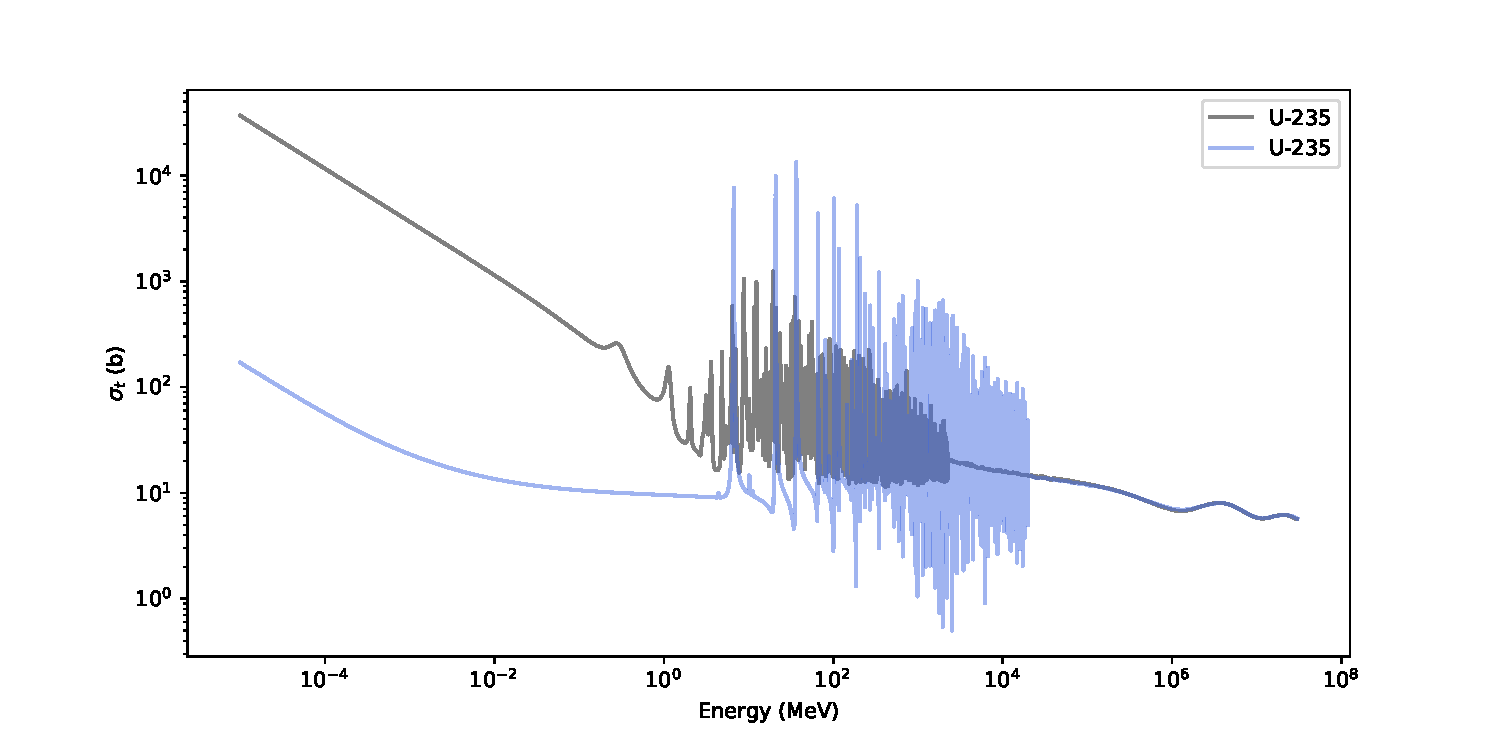
\includegraphics[width=0.85\linewidth]{\figpath/U235-8-XST}
          \caption{Uranium 235 and 238 total microscopic cross sections as a function of energy. Data provided through the ENDF-8.0 nuclear reaction data library \cite{ENDF8}.}
          \label{fig:NTT:Cross Section plot}
        \end{figure}

        The complicated dependence on energy would require hundreds of thousands of energy points to faithfully represent all the resonances of interest in thermal reactors.
        Modeling of this many energy points in whole-core simulations would be computationally impractical.
        The multigroup eigenvalue transport equation can be found by integrating the \cref{eq:NTT:Eigenvalue Transport Problem} over an energy energy interval $[E_{g}, E_{g-1})$, where $E_{g} > E_{g-1}$.
        \begin{aequation}\label{eq:NTT:MGEV Transport Problem w/ Anisotropic XS}
          \left[\dir\vdot\grad + \xst[\loc,\dir]\right]\aflux
            = \rfourpi\Bigg[&\suml[\gprime=1][G]\intl[\fourpi]\xss[][\loc][\dir,\dirprime]\aflux[\loc][\dirprime][\gprime]\ddirprime \\
            + &\frac{\spect}{\keff}\suml[\gprime=1][G]\nufis[\loc,\dir]\sflux[\loc]\Bigg]
        \end{aequation}
        \begin{equation*}
          \forall\loc, \quad \forall\dir\in\fourpi,\quad \forall g\in\{1,2,\ldots,G\},
        \end{equation*}
        where the multigroup quantities are defined by
        \begin{subequations}\label[subeqs]{eqs:NTT:Multigroup Quantities Anisotropic}
          \begin{equation}\label{eq:NTT:Multigroup Angular Flux}
            \aflux \defined \intl[E_g][E_{g-1}]\AngularFlux(\loc,\dir,E)\dif{E},
          \end{equation}
          \begin{equation}\label{eq:NTT:Multigroup Spectrum}
            \spect \defined \intl[E_g][E_{g-1}]\Spectrum(\loc,E)\dif{E},
          \end{equation}
          \begin{equation}\label{eq:NTT:Multigroup Total Cross Section Anisotropic}
            \xst[\loc,\dir] \defined \frac{\intl[E_{g}][E_{g-1}]\CrossSection_{t}(\loc,E)\AngularFlux(\loc,\dir,E)\dif{E}}{\aflux},
          \end{equation}
          \begin{equation}\label{eq:NTT:Multigroup Fission Cross Section Anisotropic}
            \nufis[\loc,\dir][g] \defined \frac{\intl[E_{g}][E_{g-1}]\nu\CrossSection_{f}(\loc,E)\AngularFlux(\loc,\dir,E)\dif{E}}{\aflux},
          \end{equation}
          \begin{equation}\label{eq:NTT:Multigroup Scattering Cross Section Anisotropic}
            \xss[][\loc][\dir,\dirprime] \defined \frac{\intl[E_{g}][E_{g-1}]\intl[E_{\gprime}][E_{\gprime-1}]\CrossSection_{s}(\loc,\dirprime\vdot\dir,\Eprime\to E)\AngularFlux(\loc,\dirprime,\Eprime)\dif{\Eprime}\dif{E}}{\aflux[\loc][\dirprime][\gprime]}.
          \end{equation}
        \end{subequations}

        By defining the cross sections in this way, no approximations have been made, and the reaction rates of each energy group are preserved.
        However, this approach has two issues: the cross sections are dependent on the angular flux which is not known \textit{a priori}, and have dependence on the neutron direction of flight.
        Generally, the dependence on the angular flux is addressed by solving a \emph{spatially} simplified problem to generate a continuous or fine-group neutron energy spectrum.
        This spectrum is then used as the weighting function (in place of $\aflux$) to ``collapse'' the cross sections into coarser multigroup values \cite{Knott2010}.
        This introduces an approximation into the transport equation.

        To eliminate the directional dependence of the multigroup cross sections, an additional approximation is made: isotropic angular flux spectrum,
        \begin{equation}\label{eq:NTT:Multigroup Isotropic Spectrum}
          \AngularFlux(\loc,\dir,E) \approx \rfourpi\FluxSpectrum(\loc, E).
        \end{equation}
        Using this approximate angular flux as the weighting function for multigroup cross sections in \cref{eq:NTT:MGEV Transport Problem w/ Anisotropic XS,eqs:NTT:Multigroup Quantities Anisotropic} can be simplified to
        \begin{aequation}\label{eq:NTT:MGEV Transport Problem}
          \left[\dir\vdot\grad + \xst\right]\aflux = \rfourpi\Bigg[&\suml[\gprime=1][G]\intl[\fourpi]\xss\aflux[\loc][\dirprime][\gprime]\ddirprime\\
              + \frac{\spect}{\keff}&\suml[\gprime=1][G]\nufis\intl[\fourpi]\aflux[\loc][\dirprime][\gprime]\ddirprime\Bigg],
        \end{aequation}
        \begin{equation*}
          \forall\loc, \quad \forall\dir\in\fourpi,\quad \forall g\in\{1,2,\ldots,G\},
        \end{equation*}
        where the approximated multigroup cross sections are defined as
        \begin{subequations}\label[subeqs]{eqs:NTT:Multigroup Cross Sections}
          \begin{equation}\label{eq:NTT:Multigroup Total Cross Section}
            \xst \defined \frac{\intl[E_{g}][E_{g-1}]\CrossSection_{t}(\loc,E)\FluxSpectrum(\loc,E)\dif{E}}{\intl[E_{g}][E_{g-1}]\FluxSpectrum(\loc,E)\dif{E}},
          \end{equation}
          \begin{equation}\label{eq:NTT:Multigroup Fission Cross Section}
            \nufis[\loc][g] \defined \frac{\intl[E_{g}][E_{g-1}]\nu\CrossSection_{f}(\loc,E)\FluxSpectrum(\loc,E)\dif{E}}{\intl[E_{g}][E_{g-1}]\FluxSpectrum(\loc,E)\dif{E}},
          \end{equation}
          \begin{equation}\label{eq:NTT:Multigroup Scattering Cross Section}
            \xss \defined \frac{\intl[E_{g}][E_{g-1}]\intl[E_{\gprime}][E_{\gprime-1}]\CrossSection_{s}(\loc,\dirprime\vdot\dir,\Eprime\to E)\FluxSpectrum(\loc,\Eprime)\dif{\Eprime}\dif{E}}{\intl[E_{\gprime}][E_{\gprime-1}]\FluxSpectrum(\loc,\Eprime)\dif{\Eprime}}.
          \end{equation}
        \end{subequations}

        For thermal reactors, the weighting spectrum, $\FluxSpectrum(\loc, E)$, is well approximated by a spatially uniform spectrum, $\FluxSpectrum(E)$.
        This justifies the use of the spectrum of the spatially simplified system.
        However, this is not the case for other systems, such as fast reactors.
        In such systems, the spatial dependence of the weighting spectrum plays is important to capture accurately, and the above methods cannot be used.
      }

      \subsubsection{Spatial Discretization}{\label{sssec:NTT:Spatial Discretization}
        Nearly all computational transport methods involve some form of spatial discretization.
        Reactor designs include many different material regions, and nearly all simulation tools will discretize the spatial domain into these different material regions.
        Deterministic methods will generally apply a finer meshing within these material regions, to discretize them into \emph{transport cells}.
        For the purposes of this work, a cell $\mathcal{R}_i$ is indexed with $i$.
        A visualization of the material and hypothetical meshing of a characteristics based transport method for a single pin-cell are shown in \cref{fig:NTT:Pin Cell}.
        In deterministic codes, the typical assumption is that material properties (cross sections) are constant within each computational cell.

        \begin{figure}[h]
          \centering
          \begin{subfigure}[t]{0.45\linewidth}
            \centering
            \def\svgwidth{\linewidth}
            \input{\figpath/PinCell.pdf_tex}
            \caption{Material regions}
            \label{fig:NTT:Pin Cell Materials}
          \end{subfigure}%
          \hfill
          \begin{subfigure}[t]{0.45\linewidth}
            \centering
            \def\svgwidth{\linewidth}
            \input{\figpath/PinCellMesh.pdf_tex}
            \caption{Hypothetical computational cell mesh}
            \label{fig:NTT:Pin Cell Mesh}
          \end{subfigure}
          \caption{Material and mesh spatial discretization examples for a single pin cell.}
          \label{fig:NTT:Pin Cell}
        \end{figure}
      }

      \subsubsection{Directional Discretization}{\label{sssec:NTT:Directional Discretization}
        %%% Discrete Ordinates Quantities %%%
\DeclareDocumentCommand{\mprime}{}{m^{\prime}}
\DeclareDocumentCommand{\dirm}{ O{m} }{\dir_{#1}}
\DeclareDocumentCommand{\wt}{ O{m} }{\Weight_{#1}}

% Quadrature set
\DeclareDocumentCommand{\angquad}{ O{N} }{ \mathcal{M}_{#1} }

% Cross-Sections
\DeclareDocumentCommand{\xss}{ o O{\loc} O{ m^{\prime}\!\to m} O{\gprime\!\to g} }{
    \IfNoValueOrEmptyTF{#1}
    {\xs[s,#3][#2][#4]}
    {\xs[s,#1][#2][#4]}
}

% Flux
\DeclareDocumentCommand{\aflux}{ O{\loc} O{m} O{g}}{\ensuremath{\AngularFlux^{#3}_{#2}\!\left(#1\right)}}

% Source
\DeclareDocumentCommand{\source}{ O{\loc} O{m} O{g} }{\ensuremath{q^{#3}_{#2}\!\left(#1\right)}}


        Typically, the directional variable cannot be treated exactly in deterministic methods.
        There are two common methods of approximating the solution as a function of direction $\dir$:
        \begin{enumerate}
          \item{\acf{PN} Expansion}
          \item{\acf{SN}}
        \end{enumerate}

        \paragraph{\acf{PN} Expansion} {
          Expansion in spherical harmonics, often referred to as \acs{PN}, is one of the oldest transport methods, where $N$ indicates the order of the expansion.
          In this method, the angular flux is expanded as a linear combination of spherical harmonics moments:
          \begin{equation}\label{eq:PN:PN Infinite Expansion}
            \aflux = \suml[l=0][\infty]\suml[n=-l][l]\afluxmom\SH,
          \end{equation}
          where the spherical harmonics,$\SH$, are defined by \cref{eqs:NTT:Spherical Harmonics Definitions}.
          No approximation has been introduced at this point, but in practice this series is truncated at some finite number $N$:
          \begin{equation}\label{eq:PN:PN Expansion}
            \aflux \approx \suml[l=0][N]\suml[n=-l][l]\afluxmom\SH.
          \end{equation}

          The \ac{PN} equations can be found by multiply the multi-group transport equation (\cref{eq:NTT:MGEV Transport Problem}) by $\SH$ for each valid $(l,n)$ pair under the specified order, and integrating over $\fourpi$.
          This yields a system of $(N+1)^2$ equations for each energy group; the number of equations increases quadratically with increasing orders, making \ac{PN} methods less feasible for large calculations.
        }

        \paragraph{\acf{SN}}{
          The \acf{SN} method is a discretization of the directional variable $\dir$ by a quadrature.
          \begin{subequations}\label[subeqs]{eqs:NTT:Directional Quadrature}
            Let the $\angquad$ be the set of discrete directions, and weights,
            \begin{equation}\label{eq:NTT:Directional Quadrature Definition}
              \angquad \defined \left\{\dirm \in \{\dir_1,\dir_2,\ldots,\dir_N\}, \wt \in \{\wt[1], \wt[2], \ldots,\wt[N]\}\right\},
            \end{equation}
            such that a directional integration can be approximated as
            \begin{equation}\label{eq:NTT:Directional Quadrature Integration}
              \intl[\fourpi]f(\dir)\ddir \approx \fourpi\suml[m\in\angquad]\wt f(\dirm),
            \end{equation}
            where
            \begin{equation}\label{eq:NTT:Directional Quadrature Weight Sum}
              \suml[m\in\angquad]\wt = 1.
            \end{equation}
          \end{subequations}

          There are two common forms of quadrature sets that are commonly used in transport calculations: level-symmetric and product quadratures.
          The level-symmetric quadratures include directions that are evenly distributed over the unit-sphere; this is optimal in situations where each direction has similar variation.
          However, typical reactor designs have significantly less variation in the axial ($z$) direction which fuel rods are oriented along.
          In this situation, neutrons with directions close to the $z$-axis are modeled poorly because there are few azimuthal angles at these polar levels, as is demonstrated in \cref{fig:NTT:S8 Quadrature}.
          These steep polar angles are important in reactor analysis due to self-shielding effects, which are strongly dependent on polar angle. % [CITATION].

          Product quadratures are generated by a multiplicative combination of separate quadrature sets in the azimuthal and polar directions.
          The azimuthal quadrature set is generated over the domain $[0,2\pi]$, while the polar quadrature set is generated for the polar cosine, $\mu$, over the domain $[-1,1]$.
          This quadrature generation technique does not suffer from the same issue for steep polar directions, as each polar level has the same number of azimuthal directions.
          A common choice for the azimuthal quadrature generation is the Chebyshev quadrature, which gives evenly spaced azimuthal angles with equal weights.
          The polar cosine quadrature set typically uses a Gauss-Legendre quadrature, or an optimized quadrature such as the Tabuchi-Yamamoto quadrature \cite{TabuchiYamamotoQuad}.
          \Cref{fig:NTT:ChebyshevGauss Quadrature} shows an example of a product quadrature's set of directions using a Chebyshev azimuthal quadrature and Gauss-Legendre polar quadrature.

          \begin{figure}[h]
            \centering
            \begin{subfigure}[t]{0.45\linewidth}
              \centering
              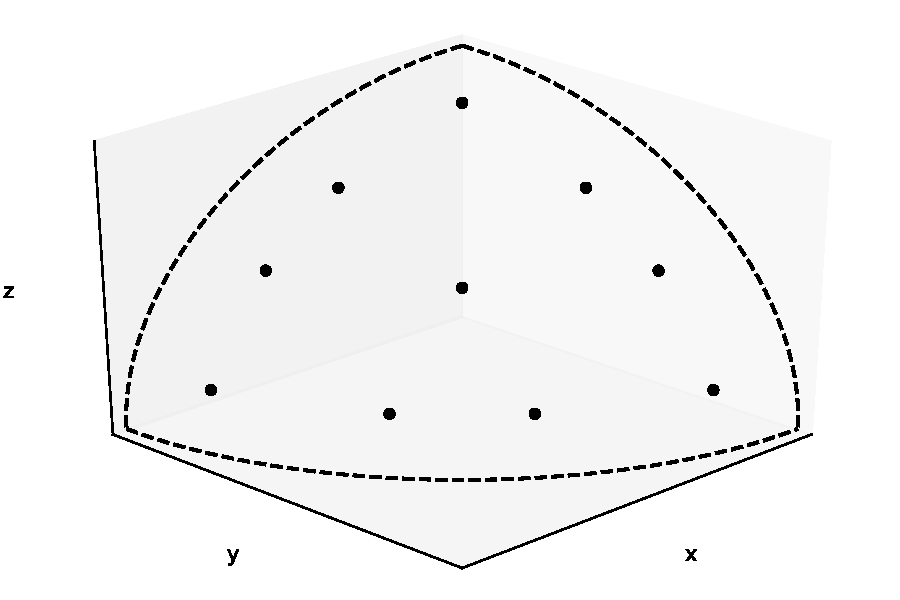
\includegraphics[width=\linewidth]{S8-Quadrature}
              \caption{Level-Symmetric Quadrature ($S_8$)}
              \label{fig:NTT:S8 Quadrature}
            \end{subfigure}%
            \hfill
            \begin{subfigure}[t]{0.45\linewidth}
              \centering
              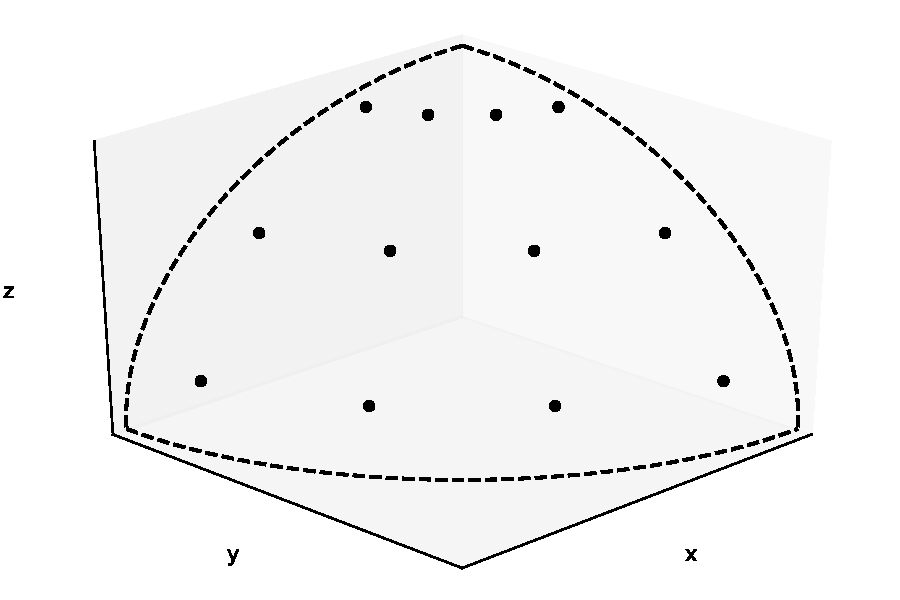
\includegraphics[width=\linewidth]{ChebyshevGauss}
              \caption{Chebyshev-Gauss Product Quadrature with 4 azimuthal and 3 polar angles}
              \label{fig:NTT:ChebyshevGauss Quadrature}
            \end{subfigure}
            \caption{(a) Level-Symmetric and (b) product quadrature direction set examples shown for a single octant of the unit-sphere.}
            \label{fig:NTT:Quadrature Examples}
          \end{figure}
        }
      }
    }
  }

  \section{State-of-the-Art 3-D Computational Transport Methods}{\label{sec:NTT:3-D Transport Methods}
    Until recently, whole-core neutronics calculations were carried out primarily through a two-step procedure.
    First, a transport method was used to compute homogenized cross section data for assemblies, and then 3-D diffusion was used to solve the problem.
    More recently, however, research has been focused on a one-step approach, so called direct whole-core transport.
    In such an approach, the 3-D reactor is directly modeled using transport methods.
    There are many different transport methods which are currently being researched; this section seeks to give an overview of several state-of-the-art 3-D transport methods.

    \subsection{S\texorpdfstring{$P_N$}{PN}}{\label{ssec:3T:SPN}
      \DeclareDocumentCommand{\xstr}{ m }{\CrossSection_{tr,#1}}
      \DeclareDocumentCommand{\xsa}{}{\CrossSection_{a}}
      \DeclareDocumentCommand{\xst}{}{\CrossSection_{t}}
      \DeclareDocumentCommand{\xss}{ m }{\CrossSection_{s,#1}}
      \DeclareDocumentCommand{\fluxm}{ m }{ \phi_{#1} }
      \DeclareDocumentCommand{\Q}{}{Q}
      \DeclareDocumentCommand{\D}{}{}

      The \acf{SPN} method was introduced by \citet{SPN} in 1961, and was seen as a middle ground between diffusion and transport \cite{Mcclarren2010}.
      The \ac{SPN} equations were first derived by examining the form of the 1-D \ac{PN} equations; in fact, the 1-D \ac{SPN} and \ac{PN} equations are equivalent.
      While the original derivation \citet{SPN} lacked theoretical justification, the \ac{SPN} method has since been shown to be an asymptotic correction to standard diffusion theory \cite{Larsen2010}.

      The mono-energetic planar geometry \ac{PN} equations can be written as
      \begin{subequations}\label[subeqs]{eqs:eqs}
        \begin{equation}\label{eq:SPN:Planar PN}
          \deriv{}{z}\left[\frac{l}{2l+1}\fluxm{l-1} + \frac{l+1}{2l+1}\fluxm{l+1}\right] + \xst\fluxm{l} = \xss{l}\fluxm{l} + \Q\delta_{l,0}, \quad\text{for}\quad 0\leq l\leq N,
        \end{equation}
        where $\xss{l}$ is the lth order scattering moment and $\Q$ is either an external source or fission source.
      \end{subequations}
      The expansion is generally truncated by assuming that $\fluxm{N+1}=0$.

      The 1-D $P_1$ equation can be written as
      \begin{equation}\label{eq:SPN:P1}
        -\deriv{}{z}\D\deriv{}{z}\fluxm{0} + \xst\fluxm{0} = \xss{0}\fluxm{0} + \Q,
      \end{equation}
      where
      \begin{equation}\label{eq:SPN:Diffusion Coefficient}
        \D \defined \frac{1}{3(\xst-\xss{1})}.
      \end{equation}
      The 3-D $P_1$ equations simply replace the derivative term operator of \cref{eq:SPN:P1} with the 3-D diffusion operator,
      \[
        \deriv{}{z}\D\deriv{}{z} \to \grad\vdot\D\grad,
      \]
      yielding the 3-D $P_1$ (diffusion) equation:
      \begin{equation}\label{eq:SPN:3D Diffusion}
        -\grad\vdot\D\grad\fluxm{0} + \xst\fluxm{0} = \xss{0}\fluxm{0} + \Q.
      \end{equation}

      This simple relation between 1-D and 3-D equations only holds for the special $P_1$ case.
      The \ac{SPN} method uses a similar modification for higher-order $P_N$ equations.
      This results in some lost accuracy compared to \ac{PN}, but the \ac{SPN} equations are significantly simpler to solve \cite{SPN,Mcclarren2010}.
      Unlike \ac{PN}, \ac{SPN} equations do not converge to the transport solution as $N\to\infty$, but do generally have higher accuracy than diffusion (for orders of $N > 1$).
      Generally, S$P_3$ or S$P_5$ are considered to have sufficient accuracy, and are generally less computationally intensive than transport methods.

      The mono-energetic \ac{SPN} equations can be written as
      \begin{subequations}\label[subeqs]{eqs:SPN:SPN}
        \begin{equation}\label{eq:SPN:SPN 0}
          -\grad\vdot\frac{1}{3\xstr{1}}\grad\fluxm{0} -\grad\vdot\frac{2}{3\xstr{1}}\grad\fluxm{2} + \xstr{0}\fluxm{0} = \Q,
        \end{equation}
        \begin{aequation}\label{eq:SPN:SPN N}
          &-\grad\vdot\left(\frac{n(n-1)}{(2n+1)(2n-1)\xstr{n-1}}\right)\grad\fluxm{n-2}\\
          &-\grad\vdot\left(\frac{(n+1)(n+2)}{(2n+1)(2n+3)\xstr{n+1}}\right)\grad\fluxm{n+2}\\
          &-\grad\vdot\left(\frac{n^2}{(2n+1)(2n-1)\xstr{n-1}} + \frac{(n+1)^2}{(2n+1)(2n+3)\xstr{n+1}}\right)\grad\fluxm{n}\\
          &+\xstr{n}\fluxm{n} = 0, \quad{\text{for}\quad n=2,4,...,N-1},
        \end{aequation}
        where
        \begin{equation}\label{eq:SPN:xstr}
          \xstr{n} \defined \CrossSection_t - \CrossSection_{s,n}.
        \end{equation}
      \end{subequations}

      [CURRENT RESEARCH]
    }

    % Here just to make sure previous macros didn't screw anything up
    %%% Multi-group Energy quantities %%%
\DeclareDocumentCommand{\gprime}{}{g^{\prime}}
% Cross-sections
\DeclareDocumentCommand{\xs}{ O{t} O{\loc} O{g}}{\ensuremath{\CrossSection_{#1}^{#3}(#2)}}
\DeclareDocumentCommand{\xst}{ O{\loc} O{g} }{\xs[t][#1][#2]}
\DeclareDocumentCommand{\xsa}{ O{\loc} O{g} }{\xs[a][#1][#2]}
\DeclareDocumentCommand{\xsf}{ O{\loc} O{\gprime} }{\xs[f][#1][#2]}
\DeclareDocumentCommand{\xss}{ o O{\loc} O{\dirprime\vdot\dir} O{\gprime \to g} }{
    \IfNoValueOrEmptyTF{#1}
    {\xs[s][#2,#3][#4]}
    {\xs[s,#1][#2][#4]}
}
\DeclareDocumentCommand{\spect}{ O{\loc} O{g} }{\ensuremath{\Spectrum^{#2}(#1)}}
\DeclareDocumentCommand{\nufis}{ O{\loc} O{\gprime} }{ \ensuremath{\nu\xsf[#1][#2]}}
\DeclareDocumentCommand{\D}{ O{\loc} O{g} }{\ensuremath{D^{#2}(#1)}}

% Flux
\DeclareDocumentCommand{\aflux}{ O{\loc} O{\dir} O{g} }{\ensuremath{\AngularFlux^{#3}(#1,#2)}}
\DeclareDocumentCommand{\sflux}{ O{\loc} O{\gprime} }{\ensuremath{\ScalarFlux^{#2}(#1)}}
\DeclareDocumentCommand{\current}{ O{\loc} O{g} }{\ensuremath{\Current^{#2}(#1)}}
\DeclareDocumentCommand{\fluxmoma}{ O{\ell} O{n} O{\loc} O{g} }{\ensuremath{\ScalarFlux^{#2,#4}_{#1}(#3)}}

% Source
\DeclareDocumentCommand{\source}{ O{\loc} O{\dir} O{g} }{\ensuremath{q^{#3}(#1,#2)}}
\DeclareDocumentCommand{\sourcemoma}{ O{\ell} O{n} O{\loc} O{g} }{\ensuremath{q^{#2,#4}_{#1}(#3)}}

    %%% Discrete Ordinates Quantities %%%
\DeclareDocumentCommand{\mprime}{}{m^{\prime}}
\DeclareDocumentCommand{\dirm}{ O{m} }{\dir_{#1}}
\DeclareDocumentCommand{\wt}{ O{m} }{\Weight_{#1}}

% Quadrature set
\DeclareDocumentCommand{\angquad}{ O{N} }{ \mathcal{M}_{#1} }

% Cross-Sections
\DeclareDocumentCommand{\xss}{ o O{\loc} O{ m^{\prime}\!\to m} O{\gprime\!\to g} }{
    \IfNoValueOrEmptyTF{#1}
    {\xs[s,#3][#2][#4]}
    {\xs[s,#1][#2][#4]}
}

% Flux
\DeclareDocumentCommand{\aflux}{ O{\loc} O{m} O{g}}{\ensuremath{\AngularFlux^{#3}_{#2}\!\left(#1\right)}}

% Source
\DeclareDocumentCommand{\source}{ O{\loc} O{m} O{g} }{\ensuremath{q^{#3}_{#2}\!\left(#1\right)}}

    %%% MOC quantities %%%
% Geometric
\DeclareDocumentCommand{\Length}{}{s}
\DeclareDocumentCommand{\NormalizedLength}{}{t}
\DeclareDocumentCommand{\len}{ O{} }{\Length_{#1}}
\DeclareDocumentCommand{\segl}{ O{mki} }{\Length_{#1}}
\DeclareDocumentCommand{\nlen}{ O{m} }{\NormalizedLength_{#1}}
\DeclareDocumentCommand{\nsegl}{ O{mki} }{\NormalizedLength_{#1}}

\DeclareDocumentCommand{\centroid}{ O{\loc} O{i} }{#1_{#2}^{\text{c}}}
\DeclareDocumentCommand{\locIn}{ O{\loc} O{mki} }{{#1}_{#2}^{\text{in}}}
\DeclareDocumentCommand{\locOut}{ O{\loc} O{mki} }{{#1}_{#2}^{\text{out}}}
\DeclareDocumentCommand{\locCent}{ O{\loc} O{mki} }{{#1}_{#2}^{\text{c}}}
\DeclareDocumentCommand{\M}{ o O{i}}{%
    \IfNoValueOrEmptyTF{#1}
        {\vec{M}_{#2}}
        {M_{#2,#1}}
}
\DeclareDocumentCommand{\C}{o O{i} O{g}}{%
    \IfNoValueOrEmptyTF{#1}
        {\vec{C}_{#2}^{#3}}
        {C_{#2,#1}^{#3}}
}


% Integration
\DeclareAutoPairedDelimiter{\MOCTrackIntegral}{\langle}{\rangle_{mki}}
\DeclareAutoPairedDelimiter{\MOCSingleAngleIntegral}{\langle}{\rangle_{mi}}
\DeclareAutoPairedDelimiter{\MOCIntegral}{\langle}{\rangle_{i}}

% Cross-sections
\DeclareDocumentCommand{\xs}{ O{t} O{i} O{g}}{\ensuremath{\CrossSection_{#1,#2}^{#3}}}
\DeclareDocumentCommand{\xst}{ O{i} O{g} }{\xs[t][#1][#2]}
\DeclareDocumentCommand{\xsa}{ O{i} O{g} }{\xs[a][#1][#2]}
\DeclareDocumentCommand{\xsf}{ O{i} O{\gprime} }{\xs[f][#1][#2]}
\DeclareDocumentCommand{\xss}{ o O{i} O{m'\to m} O{\gprime \to g} }{
    \IfNoValueOrEmptyTF{#1}
    {\xs[s][#2,#3][#4]}
    {\xs[s,#1][#2][#4]}
}

\DeclareDocumentCommand{\spect}{ O{i} O{g} }{\ensuremath{\Spectrum^{#2}_{#1}}}
\DeclareDocumentCommand{\nufis}{ O{i} O{\gprime} }{ \ensuremath{\nu\xsf[#1][#2]}}
\DeclareDocumentCommand{\D}{ O{i} O{g} }{\ensuremath{D^{#2}_{#1}}}
\DeclareDocumentCommand{\opt}{ O{m} O{g} }{\OpticalThickness_{#1}^{#2}}
\DeclareDocumentCommand{\segopt}{ O{mki} O{g} }{\opt[#1][#2]}

% MOC Parameters
\DeclareDocumentCommand{\tA}{ O{a} }{\ensuremath{\delta\!A_{#1}}}
\DeclareDocumentCommand{\Weight}{}{w}
\DeclareDocumentCommand{\wt}{ O{m} }{\Weight_{#1}}
\DeclareDocumentCommand{\wtbar}{ O{m} }{\overline{\Weight}_{#1}}
\DeclareDocumentCommand{\renorm}{ O{i} }{\ensuremath{\xi_{#1}}}

% Flux
\DeclareDocumentCommand{\aflux}{ O{mki} O{g} O{\len} }{
    \IfNoValueOrEmptyTF{#3}
    {\AngularFlux^{#2}_{#1}}
    {\ensuremath{\AngularFlux^{#2}_{#1}\!\left(#3\right)}}
}
\DeclareDocumentCommand{\afluxin}{ O{mki} O{g} }{\AngularFlux^{#2,\text{in}}_{#1}}
\DeclareDocumentCommand{\afluxout}{ O{mki} O{g} }{\AngularFlux^{#2,\text{out}}_{#1}}
\DeclareDocumentCommand{\sflux}{ O{g} O{i} }{\ScalarFlux_{#2}^{#1}}
\DeclareDocumentCommand{\current}{ O{i} O{g} }{\Current^{#2}_{#1}}
\DeclareDocumentCommand{\tfluxF}{ O{mki} O{g} }{ \overline{\AngularFlux}_{#1}^{#2} }          % Average flux-moment along track
\DeclareDocumentCommand{\tfluxL}{ O{mki} O{g} }{  \widehat{\AngularFlux}_{#1}^{#2} }          % Linear flux-moment along track
\DeclareDocumentCommand{\dflux}{ O{mki} O{g} }{ \Delta\AngularFlux_{#1}^{#2} }                % Difference of angular flux along track
\DeclareDocumentCommand{\sfluxF}{ O{i} O{g} }{ \overline{\ScalarFlux}_{#1}^{#2} }             % Average scalar flux
% \DeclareDocumentCommand{\sfluxL}{ o O{i} O{g} }{ % Linear expansion coeff (Scalar Flux)
%     \IfNoValueOrEmptyTF{#1}
%         {\lvec{\widehat{\ScalarFlux}}_{#2}^{#3}}
%         {\widehat{\ScalarFlux}_{#2,#1}^{#3}}
% }
\DeclareDocumentCommand{\sfluxL}{ O{i} O{g} o }{ % Linear expansion coeff (Scalar Flux)
    \IfNoValueOrEmptyTF{#3}
        {\lvec{\widehat{\ScalarFlux}}_{#1}^{#2}}
        {\widehat{\ScalarFlux}_{#1,#3}^{#2}}
}
% \DeclareDocumentCommand{\sfluxL}{ m O{i} O{g} }{\widehat{\ScalarFlux}_{#2,#1}^{#3} }          % Linear expansion coeff (Scalar flux)
\DeclareDocumentCommand{\afluxmom}{ O{\ell} O{n} O{i} O{\gprime} }{\FluxMoment_{#3,#1}^{#4,#2}}

% Source
\DeclareDocumentCommand{\source}{ O{mki} O{g} O{\len} }{\ensuremath{q^{#2}_{#1}\!\left(#3\right)}}
\DeclareDocumentCommand{\tsrcF}{ O{mki} O{g} }{ \overline{q}_{#1}^{#2} }          % Average source along track
\DeclareDocumentCommand{\tsrcL}{ O{mi} O{g} }{ \widehat{q}_{#1}^{#2} }          % Linear source along track
\DeclareDocumentCommand{\src}{ O{i} O{g} }{ \Source_{#1}^{#2}}                          % Generic source
\DeclareDocumentCommand{\srcF}{ O{i} O{g} }{ q_{#1}^{#2} }             % Average source
\DeclareDocumentCommand{\srcL}{ o O{i} O{g} }{ % Linear expansion coeff (Source)
    \IfNoValueOrEmptyTF{#1}
        {\lvec{\widehat{q}}_{#2}^{#3}}
        {\widehat{q}_{#2,#1}^{#3}}
}

% Linear source operators / functions
\DeclareDocumentCommand{\FluxToSource}{ O{g} }{\mathcal{S}^{#1}}

    \subsection{2D/1D Methods}{\label{ssec:3T:2D/1D Methods}
      The 2D/1D methods were first developed by researchers at \ac{KAIST} \cite{Cho2002} and \ac{KAERI} \cite{DeCART}, in the CRX and DeCART codes, respectively.
      Though different, these two methods followed the same fundamental approach to solving 3-D reactor transport problems:
      \begin{enumerate}
        \item{Divide the core into separate axial slices/planes,}
        \item{Perform 2-D transport calculations within each plane,}
        \item{Couple the planes with transverse leakages.}
      \end{enumerate}
      These methods were based on the assumption that reactors may be very heterogeneous in the radial direction, but in the axial direction they are relatively homogeneous.
      The primary difference between these two methods is in the transverse leakage terms; in CRX the transverse leakages are anisotropic, but in DeCART the leakages are isotropic.
      To distinguish these methods, they will be referred to as anisotropic and isotropic 2D/1D methods.

      Following the relative success of these methods, other research groups have followed in their paths.
      nTRACER \cite{Jung2009}, and MPACT \cite{MPACT2016} used the isotropic 2D/1D method.
      The STREAM \cite{Zheng2017}, and APOLLO3 \cite{Faure2018} have also implemented 2D/1D methods.

      \citet{Stimpson2015} implemented an anisotropic 2D/1D method in MPACT using a Fourier expansion of the azimuthal angles for the axial and radial transverse leakages.
      \citet{Jarrett2018} further improved upon \citetp{Stimpson2015} work by introducing a 2D/1D method using $P_3$ in the axial direction.
      2D/1D methods are fundamentally based on the idea that heterogeneity in the axial direction is very low;
      thus, in cases where this is not true these methods have been observed to break down, or yield incorrect solutions.

      \DeclareDocumentCommand{\aflux}{}{\psi}
      \DeclareDocumentCommand{\xst}{ O{t} }{\Sigma_{#1}}
      \DeclareDocumentCommand{\mxst}{ O{t} }{\widetilde{\Sigma}_{#1}}
      \DeclareDocumentCommand{\dir}{}{\vec{\Omega}}
      \DeclareDocumentCommand{\rloc}{}{\loc_{xy}}
      \DeclareDocumentCommand{\TL}{}{\widetilde{J}}
      \DeclareDocumentCommand{\L}{}{\widetilde{L}}

      \subsubsection{Derivation}{\label{sssec:3T:Derivation}
        The details of the 2D/1D equations have implications on results in \cref{ch:Improved Linear Source Formulation for Multi-physics and 2D/1D Applications}.
        In this section, the 2D/1D equations are derived.
        Begin with the mono-energetic transport equation
        \begin{equation}\label{eq:2D/1D:Transport}
          \dir\vdot\grad\aflux(\loc,\dir) + \xst(\loc)\aflux(\loc,\dir) = \frac{Q(\loc)}{\fourpi},
        \end{equation}
        where $Q(\loc)$ is the source.

        The 2D/1D methods divide the transport equation into radial (2-D) and axial (1-D) equations.
        The streaming term, $\dir\vdot\grad\aflux$ can be divided into the radial and axial components:
        \begin{equation}\label{eq:2D/1D:Streaming Split}
          \dir\vdot\grad\aflux = (\dir\vdot\grad)_{xy}\aflux + \PolarCos\pderiv{\aflux}{z}.
        \end{equation}
        The radial equation can be found by first separating the axial derivative from the streaming term:
        \begin{equation}\label{eq:2D/1D:Radial Eqn. 1}
          \left[(\dir\vdot\grad)_{xy} + \xst\right]\aflux(\loc,\dir) = \frac{Q(\loc)}{\fourpi} - \PolarCos\pderiv{\aflux}{z}.
        \end{equation}
        \Cref{eq:2D/1D:Radial Eqn. 1} is then integrated over an axial plane $k$, over the interval $[z_{k-1/2}, z_{k+1/2}]$, yielding
        \begin{subequations}\label[subeqs]{eqs:2D/1D:Radial Eqn.}
          \begin{equation}\label{eq:2D/1D:Radial Eqn.}
            \left[(\dir\vdot\grad)_{xy} + \xst[t,k](\rloc)\right]\aflux_k(\rloc,\dir) = \frac{Q_k(\rloc)}{\fourpi} - \TL_{z,k}(\rloc,\dir),
          \end{equation}
          where
          \begin{equation}\label{eq:2D/1D:Radial Flux}
            \aflux_k(\rloc,\dir) \defined \frac{1}{h_k}\intl[z_{k-1/2}][z_{k+1/2}]\aflux(\loc,\dir)\dif{z},
          \end{equation}
          \begin{equation}\label{eq:2D/1D:Radial Source}
            Q_k(\rloc) \defined \frac{1}{h_k}\intl[z_{k-1/2}][z_{k+1/2}]Q(\loc,\dir)\dif{z},
          \end{equation}
          \begin{equation}\label{eq:2D/1D:Axial TL}
            \TL_{z,k}(\rloc,\dir) = \frac{\PolarCos}{h_k}\left[\aflux(\rloc,z_{k+1/2},\dir) - \aflux(\rloc,z_{k-1/2})\right],
          \end{equation}
          and $h_k = z_{k+1/2}-z_{k-1/2}$.
        \end{subequations}
        Generally, the difference between isotropic and anisotropic 2D/1D methods is in the treatment of the transverse leakages, $\TL_{z,k}$.
        In MPACT, the axial transverse leakage is typically discretized over the coarse radial mesh (typically a pin cell), and is assumed to be isotropic.

        The axial equations are found by moving the radial streaming term to the right hand side of \cref{eq:2D/1D:Transport},
        \begin{equation}\label{eq:2D/1D:Axial Eqn. 1}
          \left[\PolarCos\pderiv{}{z} + \xst\right]\aflux(\loc,\dir) = \frac{Q(\loc)}{\fourpi} - (\dir\vdot\grad)_{xy}\aflux(\loc,\dir),
        \end{equation}
        and integrating over a radial area.
        This radial area can be a fine cell (transport cell), but is typically a coarser discretization such as a pin cell \cite{Jarrett2018}.
        Operate on \cref{eq:2D/1D:Axial Eqn. 1} by
        \[
          \frac{1}{A_{ij}}\intl[x_{i-1/2}][x_{i+1/2}]\intl[y_{j-1/2}][y_{j+1/2}](\vdot)\dif{x}\dif{y}
          =
          \frac{1}{A_{ij}}\iint_{ij}(\vdot)\dif{x}\dif{y},
        \]
        \begin{subequations}\label[subeqs]{eqs:2D/1D:Axial}
          \begin{equation}\label{eq:2D/1D:Axial}
            \left[\PolarCos\pderiv{}{z}+\xst[t,k,ij](z,\dir)\right]\aflux_{ij}(z,\dir)
              = \frac{Q_{ij}(z)}{\fourpi} - \frac{1}{A_{ij}}\suml[s\in\{N,S,E,W\}](\dir\vdot\widehat{n}_s)\aflux_{ij,s}(z,\dir),
          \end{equation}
          where
          \begin{equation}\label{eq:2D/1D:Axial XS}
            \xst[t,k,ij](z,\dir) \defined \frac{\iint_{ij}\xst[t,k](\rloc)\aflux_k(\rloc,\dir)\dif{x}\dif{y}}{\iint_{ij}\aflux_k(\rloc,\dir)\dif{x}\dif{y}},
          \end{equation}
          where $s$ indicates a surface for the cardinal directions $\{N,S,E,W\}$.
          For hexagonal pins there would instead be six directions to loop over; for simplicity this work assumes cartesian pin cells.
        \end{subequations}
        Typically the coarse cell cross sections are isotropic, but polar dependence has been investigated \cite{Jarrett2018}.

        The radial equations, \cref{eqs:2D/1D:Radial Eqn.}, are solved by a 2-D transport method, such as \ac{MOC}, while the axial equations, \cref{eqs:2D/1D:Axial}, are solved by either a transport method or approximate method such as diffusion \cite{Collins2016,Jarrett2018}.
        The radial equations yield surface fluxes on the pin faces, while the axial equations yield surface fluxes on the axial planar faces.
        The radial equations are, however, integrated over an axial plane which results in an axial flat solution within each plane.
        These methods then require many axial planes to resolve the axial behavior in a system, particularly if there is significant axial variation in the solution.
      }

      \subsubsection{Transverse Leakage Splitting}{\label{sssec:3T:Transverse Leakage Splitting}
        \Cref{eqs:2D/1D:Radial Eqn.} gives no guarantee that the right-hand-side will be a positive source.
        Negative sources present considerable challenges to iteration stability when using non-linear acceleration methods such as \ac{CMFD} \cite{Jarrett2018}.
        The transverse leakage splitting method \cite{Stimpson2015,Kelley2015} was developed to ``split'' the transverse leakage term such that the total source ($Q+\TL$) is non-negative.
        A split term, $\L_{z}$, is defined
        \begin{equation}\label{eq:2D/1D:Split Term}
          \L_z \defined -\left[\frac{Q_k(\rloc)}{\fourpi} - \TL_{z,k}(\rloc,\dir)\right],
        \end{equation}
        and is added to both sides of \cref{eq:2D/1D:Radial Eqn.}.
        The left hand side (the 2-D transport operator) cannot have a free-source term, so it is necessary to merge this split term into the cross section term.
        The angular flux is not known a priori, so a approximation is used, typically isotropic flux:
        \begin{equation}\label{eq:2D/1D:Isotropic Flux}
          \aflux_k(\rloc,\dir) \approx \frac{\phi_k(\rloc)}{\fourpi}.
        \end{equation}
        This approximation is introduced only to combine the left-hand-side leakage term into the cross section term as
        \begin{equation}\label{eq:2D/1D:Split XS}
          \mxst[t,k](\rloc) \defined \xst[t,k](\rloc) + \fourpi\frac{\L_z}{\phi_k(\rloc)}.
        \end{equation}
        The radial equation then becomes
        \begin{equation}\label{eq:2D/1D:Split Radial Eqn.}
          \left[(\dir\vdot\grad)_{xy} + \mxst[t,k](\rloc)\right]\aflux_k(\rloc,\dir) = 0.
        \end{equation}

        Because splitting introduces an approximation, it generally decreases the accuracy of the solution.
        Thus, the transverse splitting method is typically use only in cells that have a negative source.
        More recently, alternative methods have been investigated \cite{Zhao2018}, but will not be covered in this work.
      }
    }

    % Here just to make sure previous macros didn't screw anything up
    %%% Multi-group Energy quantities %%%
\DeclareDocumentCommand{\gprime}{}{g^{\prime}}
% Cross-sections
\DeclareDocumentCommand{\xs}{ O{t} O{\loc} O{g}}{\ensuremath{\CrossSection_{#1}^{#3}(#2)}}
\DeclareDocumentCommand{\xst}{ O{\loc} O{g} }{\xs[t][#1][#2]}
\DeclareDocumentCommand{\xsa}{ O{\loc} O{g} }{\xs[a][#1][#2]}
\DeclareDocumentCommand{\xsf}{ O{\loc} O{\gprime} }{\xs[f][#1][#2]}
\DeclareDocumentCommand{\xss}{ o O{\loc} O{\dirprime\vdot\dir} O{\gprime \to g} }{
    \IfNoValueOrEmptyTF{#1}
    {\xs[s][#2,#3][#4]}
    {\xs[s,#1][#2][#4]}
}
\DeclareDocumentCommand{\spect}{ O{\loc} O{g} }{\ensuremath{\Spectrum^{#2}(#1)}}
\DeclareDocumentCommand{\nufis}{ O{\loc} O{\gprime} }{ \ensuremath{\nu\xsf[#1][#2]}}
\DeclareDocumentCommand{\D}{ O{\loc} O{g} }{\ensuremath{D^{#2}(#1)}}

% Flux
\DeclareDocumentCommand{\aflux}{ O{\loc} O{\dir} O{g} }{\ensuremath{\AngularFlux^{#3}(#1,#2)}}
\DeclareDocumentCommand{\sflux}{ O{\loc} O{\gprime} }{\ensuremath{\ScalarFlux^{#2}(#1)}}
\DeclareDocumentCommand{\current}{ O{\loc} O{g} }{\ensuremath{\Current^{#2}(#1)}}
\DeclareDocumentCommand{\fluxmoma}{ O{\ell} O{n} O{\loc} O{g} }{\ensuremath{\ScalarFlux^{#2,#4}_{#1}(#3)}}

% Source
\DeclareDocumentCommand{\source}{ O{\loc} O{\dir} O{g} }{\ensuremath{q^{#3}(#1,#2)}}
\DeclareDocumentCommand{\sourcemoma}{ O{\ell} O{n} O{\loc} O{g} }{\ensuremath{q^{#2,#4}_{#1}(#3)}}

    %%% Discrete Ordinates Quantities %%%
\DeclareDocumentCommand{\mprime}{}{m^{\prime}}
\DeclareDocumentCommand{\dirm}{ O{m} }{\dir_{#1}}
\DeclareDocumentCommand{\wt}{ O{m} }{\Weight_{#1}}

% Quadrature set
\DeclareDocumentCommand{\angquad}{ O{N} }{ \mathcal{M}_{#1} }

% Cross-Sections
\DeclareDocumentCommand{\xss}{ o O{\loc} O{ m^{\prime}\!\to m} O{\gprime\!\to g} }{
    \IfNoValueOrEmptyTF{#1}
    {\xs[s,#3][#2][#4]}
    {\xs[s,#1][#2][#4]}
}

% Flux
\DeclareDocumentCommand{\aflux}{ O{\loc} O{m} O{g}}{\ensuremath{\AngularFlux^{#3}_{#2}\!\left(#1\right)}}

% Source
\DeclareDocumentCommand{\source}{ O{\loc} O{m} O{g} }{\ensuremath{q^{#3}_{#2}\!\left(#1\right)}}

    %%% MOC quantities %%%
% Geometric
\DeclareDocumentCommand{\Length}{}{s}
\DeclareDocumentCommand{\NormalizedLength}{}{t}
\DeclareDocumentCommand{\len}{ O{} }{\Length_{#1}}
\DeclareDocumentCommand{\segl}{ O{mki} }{\Length_{#1}}
\DeclareDocumentCommand{\nlen}{ O{m} }{\NormalizedLength_{#1}}
\DeclareDocumentCommand{\nsegl}{ O{mki} }{\NormalizedLength_{#1}}

\DeclareDocumentCommand{\centroid}{ O{\loc} O{i} }{#1_{#2}^{\text{c}}}
\DeclareDocumentCommand{\locIn}{ O{\loc} O{mki} }{{#1}_{#2}^{\text{in}}}
\DeclareDocumentCommand{\locOut}{ O{\loc} O{mki} }{{#1}_{#2}^{\text{out}}}
\DeclareDocumentCommand{\locCent}{ O{\loc} O{mki} }{{#1}_{#2}^{\text{c}}}
\DeclareDocumentCommand{\M}{ o O{i}}{%
    \IfNoValueOrEmptyTF{#1}
        {\vec{M}_{#2}}
        {M_{#2,#1}}
}
\DeclareDocumentCommand{\C}{o O{i} O{g}}{%
    \IfNoValueOrEmptyTF{#1}
        {\vec{C}_{#2}^{#3}}
        {C_{#2,#1}^{#3}}
}


% Integration
\DeclareAutoPairedDelimiter{\MOCTrackIntegral}{\langle}{\rangle_{mki}}
\DeclareAutoPairedDelimiter{\MOCSingleAngleIntegral}{\langle}{\rangle_{mi}}
\DeclareAutoPairedDelimiter{\MOCIntegral}{\langle}{\rangle_{i}}

% Cross-sections
\DeclareDocumentCommand{\xs}{ O{t} O{i} O{g}}{\ensuremath{\CrossSection_{#1,#2}^{#3}}}
\DeclareDocumentCommand{\xst}{ O{i} O{g} }{\xs[t][#1][#2]}
\DeclareDocumentCommand{\xsa}{ O{i} O{g} }{\xs[a][#1][#2]}
\DeclareDocumentCommand{\xsf}{ O{i} O{\gprime} }{\xs[f][#1][#2]}
\DeclareDocumentCommand{\xss}{ o O{i} O{m'\to m} O{\gprime \to g} }{
    \IfNoValueOrEmptyTF{#1}
    {\xs[s][#2,#3][#4]}
    {\xs[s,#1][#2][#4]}
}

\DeclareDocumentCommand{\spect}{ O{i} O{g} }{\ensuremath{\Spectrum^{#2}_{#1}}}
\DeclareDocumentCommand{\nufis}{ O{i} O{\gprime} }{ \ensuremath{\nu\xsf[#1][#2]}}
\DeclareDocumentCommand{\D}{ O{i} O{g} }{\ensuremath{D^{#2}_{#1}}}
\DeclareDocumentCommand{\opt}{ O{m} O{g} }{\OpticalThickness_{#1}^{#2}}
\DeclareDocumentCommand{\segopt}{ O{mki} O{g} }{\opt[#1][#2]}

% MOC Parameters
\DeclareDocumentCommand{\tA}{ O{a} }{\ensuremath{\delta\!A_{#1}}}
\DeclareDocumentCommand{\Weight}{}{w}
\DeclareDocumentCommand{\wt}{ O{m} }{\Weight_{#1}}
\DeclareDocumentCommand{\wtbar}{ O{m} }{\overline{\Weight}_{#1}}
\DeclareDocumentCommand{\renorm}{ O{i} }{\ensuremath{\xi_{#1}}}

% Flux
\DeclareDocumentCommand{\aflux}{ O{mki} O{g} O{\len} }{
    \IfNoValueOrEmptyTF{#3}
    {\AngularFlux^{#2}_{#1}}
    {\ensuremath{\AngularFlux^{#2}_{#1}\!\left(#3\right)}}
}
\DeclareDocumentCommand{\afluxin}{ O{mki} O{g} }{\AngularFlux^{#2,\text{in}}_{#1}}
\DeclareDocumentCommand{\afluxout}{ O{mki} O{g} }{\AngularFlux^{#2,\text{out}}_{#1}}
\DeclareDocumentCommand{\sflux}{ O{g} O{i} }{\ScalarFlux_{#2}^{#1}}
\DeclareDocumentCommand{\current}{ O{i} O{g} }{\Current^{#2}_{#1}}
\DeclareDocumentCommand{\tfluxF}{ O{mki} O{g} }{ \overline{\AngularFlux}_{#1}^{#2} }          % Average flux-moment along track
\DeclareDocumentCommand{\tfluxL}{ O{mki} O{g} }{  \widehat{\AngularFlux}_{#1}^{#2} }          % Linear flux-moment along track
\DeclareDocumentCommand{\dflux}{ O{mki} O{g} }{ \Delta\AngularFlux_{#1}^{#2} }                % Difference of angular flux along track
\DeclareDocumentCommand{\sfluxF}{ O{i} O{g} }{ \overline{\ScalarFlux}_{#1}^{#2} }             % Average scalar flux
% \DeclareDocumentCommand{\sfluxL}{ o O{i} O{g} }{ % Linear expansion coeff (Scalar Flux)
%     \IfNoValueOrEmptyTF{#1}
%         {\lvec{\widehat{\ScalarFlux}}_{#2}^{#3}}
%         {\widehat{\ScalarFlux}_{#2,#1}^{#3}}
% }
\DeclareDocumentCommand{\sfluxL}{ O{i} O{g} o }{ % Linear expansion coeff (Scalar Flux)
    \IfNoValueOrEmptyTF{#3}
        {\lvec{\widehat{\ScalarFlux}}_{#1}^{#2}}
        {\widehat{\ScalarFlux}_{#1,#3}^{#2}}
}
% \DeclareDocumentCommand{\sfluxL}{ m O{i} O{g} }{\widehat{\ScalarFlux}_{#2,#1}^{#3} }          % Linear expansion coeff (Scalar flux)
\DeclareDocumentCommand{\afluxmom}{ O{\ell} O{n} O{i} O{\gprime} }{\FluxMoment_{#3,#1}^{#4,#2}}

% Source
\DeclareDocumentCommand{\source}{ O{mki} O{g} O{\len} }{\ensuremath{q^{#2}_{#1}\!\left(#3\right)}}
\DeclareDocumentCommand{\tsrcF}{ O{mki} O{g} }{ \overline{q}_{#1}^{#2} }          % Average source along track
\DeclareDocumentCommand{\tsrcL}{ O{mi} O{g} }{ \widehat{q}_{#1}^{#2} }          % Linear source along track
\DeclareDocumentCommand{\src}{ O{i} O{g} }{ \Source_{#1}^{#2}}                          % Generic source
\DeclareDocumentCommand{\srcF}{ O{i} O{g} }{ q_{#1}^{#2} }             % Average source
\DeclareDocumentCommand{\srcL}{ o O{i} O{g} }{ % Linear expansion coeff (Source)
    \IfNoValueOrEmptyTF{#1}
        {\lvec{\widehat{q}}_{#2}^{#3}}
        {\widehat{q}_{#2,#1}^{#3}}
}

% Linear source operators / functions
\DeclareDocumentCommand{\FluxToSource}{ O{g} }{\mathcal{S}^{#1}}

    \subsection{Extruded 3-D Methods}{\label{ssec:3T:Extruded 3-D Methods}
      % Proteus - FEM
      % STREAM - Linear orthogonal polynomials
      % APOLLO - ?
      % Nick H. - Legendre Expansion
      % SooYoung - Diamond-Difference
    }

    \subsection{Method of Characteristics}{\label{ssec:3T:Method of Characteristics}
      The \acf{MOC} is a technique used in mathematics to solve \acp{PDE}, by transforming a \ac{PDE} into a system of \acp{ODE}.
      The method was first applied to the neutron transport problem by \citeauthor{Askew1972} in 1972 \cite{Askew1972}, but only began to see real use in the 1980's \cite{Halsall1980}.
      The \ac{MOC} transforms the transport equation into the characteristic form, by examining the equation along straight neutron paths through the spatial domain.

      By examining the equation along one of these characteristic ``tracks'' or ``rays'', the average angular flux along the track within a cell can be calculated.
      The scalar flux can then be found by collecting the average angular flux along all tracks passing through this region, in a numerical integration over space and angle.

      Like the \ac{CP} method, \ac{MOC} is able to handle completely arbitrary geometry; however, unlike the \ac{CP} method, it is also able to account for anisotropic scattering in a straightforward manner.
      Additionally, the \ac{MOC} does not produce the large matrices in realistic applications as the \ac{CP} method does.
      For problems that contain more than a few hundred cells, the \ac{MOC} is generally preferred over \ac{CP} methods \cite{Hebert2010}.

      The \ac{CDP} is a method similar to both \ac{CP} method and the \ac{MOC} \cite{Hong1999,Liu2014}.
      The \ac{CDP} uses ray-tracing to evaluate transmission probabilities between cells.
      However, it only considers transmission probabilities between cells which are traversed by a shared characteristic ray, rather than considering the transmission probability between all cells as in the \ac{CP} methods.
      This significantly cuts down on the computational resources required by traditional \ac{CP} methods.
      This method has also shown improvements over \ac{MOC} in cases with few unique geometries and constant material properties throughout the simulation; however these conditions are not applicable in problems of interest to industry.

      The \ac{MOC} is the primary subject of this thesis work.
      As such, \cref{ch:The Method of Characteristics} has been devoted to the details of the method, and \cref{sec:MOC:Ray-Tracing} expands upon the details of current ray-tracing techniques used in \ac{MOC}.
      \Cref{ch:Improved Linear Source Formulation for Multi-physics and 2D/1D Applications} details improvements made to the \ac{MOC} in this thesis work, and \cref{ch:MacroRay Three-Dimensional Ray-tracing Technique} details a newly investigated ray-tracing method.
    }
  }

  \section{Source Iteration}{\label{sec:NTT:Source Iteration}
    Generally, the $k$-eigenvalue transport problems, introduced in \cref{sec:NTT:k-Eigenvalue Problems}, are solved iteratively.
    Given an initial guess for the $k$-eigenvalue, boundary conditions, and interior flux-moments, an estimate of the source can be computed.
    A transport ``sweep'' can be performed, in which updated boundary conditions and flux-moments are computed.
    Given these updated flux-moments a new estimate of the eigenvalue can be calculated.
    This process can be repeated until the eigenvalue and flux-moments are converged within some tolerance.
    For simplicity, this process is shown for a isotropic mono-energetic, continuous-space, one-dimensional transport problem in \cref{alg:NTT:Source Iteration}.

    \begin{algorithm}[ht]
      \centering
      \caption{Source Iteration algorithm for the $k$-eigenvalue transport problem.}
      \label{alg:NTT:Source Iteration}
      \begin{algorithmic}[1]
        \State{Begin iteration $j$ with a known boundary conditions, scalar flux estimate, $\ScalarFlux^{(j)}(x)$, and a $k$-eigenvalue estimate, $\keff^{j}$.}
        \State{Perform a transport sweep:
          \begin{equation}\label{eq:NTT:Source Iteration:Transport Sweep}
            \left[\PolarCos\pderiv{}{x} + \CrossSection_t(x)\right]\AngularFlux^{(j+1)}(x,\PolarCos) = \frac{1}{2}\left[\CrossSection_s(x) + \frac{1}{\keff^{(j)}}\nu\CrossSection_f(x)\right]\ScalarFlux^{(j)}(x),
          \end{equation}
          \begin{equation*}
            \forall x\in [0,X], \quad \forall\PolarCos \in [-1, 1].
          \end{equation*}
        }
        \State{Update the scalar flux, and the eigenvalue for the next iteration:
          \begin{subequations}\label[subeqs]{eqs:NTT:Source Iteration:Update}
            \begin{equation}\label{eq:NTT:Source Iteration:Scalar Flux Update}
              \ScalarFlux^{(j+1)}(x) = \intl[-1][1]\AngularFlux^{(j+1)}(x,\PolarCos)\dif{\PolarCos} \frac{\Phi_0}{\frac{1}{X}\intl[0][X]\intl[-1][1]\AngularFlux^{(j+1)}(x',\PolarCos)\dif{\PolarCos}\dif{x'}},
            \end{equation}
            \begin{equation}\label{eq:NTT:Source Iteration:Eigenvalue Update}
              \keff^{(j+1)} = \frac{\intl[0][X]\nu\CrossSection_f\ScalarFlux^{(j+1)}(x)\dif{x}}{\intl[0][X]\CrossSection_a\ScalarFlux^{(j+1)}(x)\dif{x}}.
            \end{equation}
          \end{subequations}
        }
        \State{Repeat steps 1. - 3. until sufficient convergence.}
      \end{algorithmic}
    \end{algorithm}

    \subsection{Transport Acceleration}{\label{ssec:NTT:Transport Acceleration}
      While \cref{alg:NTT:Source Iteration} is valid, it typically converges very slowly, requiring many iterations to get reasonable results.
      In full-core calculations, a single transport sweep is typically the most computationally expensive operation and using \cref{alg:NTT:Source Iteration} is not feasible.
      There has been considerable effort in developing methods that accelerate transport calculations by using a lower-order calculation, typically based on the diffusion approximation.
      These methods often reduce the number of iterations from O(1000) to O(10) for thermal reactor systems.

      While other acceleration methods exist \cite{Hebert2017}, the most common for $k$-eigenvalue problems are \ac{NDA} methods \cite{Smith2002}, typically using the \ac{CMFD} method \cite{Smith1983}.
      \Cref{alg:NTT:NDA} lists the standard \ac{NDA} algorithm for a 1-D mono-energetic $k$-eigenvalue problem.
      The primary difference between \ac{CMFD} and \ac{NDA} is that \ac{CMFD} introduces the concept of a second, coarser spatial grid, while \ac{NDA} uses the same mesh as the transport problem.

      The \ac{CMFD} acceleration method has been shown to significantly reduce computational transport run-times \cite{Smith2002,Anistratov2011,Collins2016}.
      There have been several improvements upon the original \ac{CMFD} formulation \cite{Smith1983}, such as p\ac{CMFD} \cite{Cho2002} and od\ac{CMFD} \cite{Zhu2016}.
      The p\ac{CMFD} method preserves partial currents rather than net currents, and has been shown to be unconditionally stable for transport problems at fixed conditions \cite{Cho2002}.
      The od\ac{CMFD} method generalizes the \ac{CMFD} and p\ac{CMFD} methods by adding an artificial term to the diffusion coefficient, and has faster convergence properties than p\ac{CMFD} \cite{Zhu2016}.
      Recently, it was shown that the theoretical reason for this is the that most \ac{MOC} methods do not preserve the linear solutions of the transport equation, resulting in the need for an unphysical correction to the diffusion coefficient to account for truncation error in the transport discretization.

      Utilization of \ac{CMFD} acceleration in transport calculations with \ac{TH} feedback has not had the favorable stability and convergence properties as calculations without feedback \cite{Kochunas2017}.
      Many transport codes have required under-relaxation of the scalar flux in the iteration schemes for stability in these calculations; there is ongoing research investigating a less ad-hoc approach \cite{Kochunas2017}.
      This instability and convergence slow-down in problems with feedback has prevented full utilization of more advanced multi-level solvers \cite{Kochunas2017,Yee2018a}.

      \begin{algorithm}
        \caption{Non-linear Diffusion Acceleration (NDA) algorithm for the $k$-eigenvalue transport problem.}
        \label{alg:NTT:NDA}
        \newcommand{\ndaCurrent}[1][j]{J^{(#1)}(x)}
        \newcommand{\ndaFlux}[1][j]{\ScalarFlux^{(#1)}(x)}
        \newcommand{\ndaXST}{\CrossSection_{t}(x)}
        \newcommand{\ndaXSA}{\CrossSection_{a}(x)}
        \newcommand{\ndaNUFIS}{\nu\CrossSection_{f}(x)}
        \newcommand{\ndaD}{\frac{1}{3\ndaXST}}
        \newcommand{\ndaDHAT}{\widehat{D}^{(j)}(x)}

        \begin{algorithmic}[1]
          \State{Begin iteration $i$ with known boundary conditions, scalar flux estimate, $\ScalarFlux^{(j)}(x)$, a net current estimate, $\Current^{(j)}(x)$, and a $k$-eigenvalue estimate, $\keff$.}
          \State{Compute linear and non-linear correction factors for low-order diffusion equation:
            \begin{equation}\label{eq:NTT:NDA:Dhat}
              \ndaDHAT = \frac{\deriv{}{x}\left[\ndaCurrent + \ndaD\deriv{\ndaFlux}{x}\right]}{\ndaFlux}
            \end{equation}
          }
          \State{Solve the low-order diffusion eigenvalue problem:
            \begin{equation}\label{eq:NTT:NDA:NDA Equation}
              -\deriv{}{x}\ndaD\deriv{\ndaFlux[j+1/2]}{x}
              +\left[\ndaXSA + \ndaDHAT\right]\ndaFlux[j+1/2] = \frac{1}{\keff}\ndaNUFIS\ndaFlux[j+1/2].
            \end{equation}
          }
          \State{Perform a transport sweep using the scalar flux, and eigenvalue estimates from the low-order diffusion calculation:
            \begin{equation}\label{eq:NTT:NDA:Transport Sweep}
              \left[\PolarCos\pderiv{}{x} + \ndaXST\right]\AngularFlux^{(j+1)}(x,\PolarCos) = \frac{1}{2}\left[\CrossSection_s(x) + \frac{1}{\keff^{(j)}}\nu\CrossSection_f(x)\right]\ScalarFlux^{(j)}(x),
            \end{equation}
            \begin{equation*}
              \forall x\in [0,X], \quad \forall\PolarCos \in [-1, 1].
            \end{equation*}
          }
          \State{Update the scalar flux, current, and eigenvalue estimates for next iteration:
            \begin{subequations}\label[subeqs]{eqs:NTT:NDA:Update}
              \begin{equation}\label{eq:NTT:NDA:Scalar Flux Update}
                \ScalarFlux^{(j+1)}(x) = \intl[-1][1]\AngularFlux^{(j+1)}(x,\PolarCos)\dif{\PolarCos} \frac{\Phi_0}{\frac{1}{X}\intl[0][X]\intl[-1][1]\AngularFlux^{(j+1)}(x',\PolarCos)\dif{\PolarCos}\dif{x'}},
              \end{equation}
              \begin{equation}\label{eq:NTT:NDA:Current Update}
                \Current^{(j+1)}(x) = \intl[-1][1]\PolarCos\AngularFlux^{(j+1)}(x,\PolarCos)\dif{\PolarCos} \frac{\Phi_0}{\frac{1}{X}\intl[0][X]\intl[-1][1]\AngularFlux^{(j+1)}(x',\PolarCos)\dif{\PolarCos}\dif{x'}},
              \end{equation}
              \begin{equation}\label{eq:NTT:NDA:Eigenvalue Update}
                \keff^{(j+1)} = \frac{\intl[0][X]\nu\CrossSection_f\ScalarFlux^{(j+1)}(x)\dif{x}}{\intl[0][X]\CrossSection_a\ScalarFlux^{(j+1)}(x)\dif{x}}.
              \end{equation}
            \end{subequations}
          }
        \end{algorithmic}
      \end{algorithm}
    }
  }

  % References
  \printbibliography
}